\subsection{Modelle in der Wissenschaft}
Ein Ansatz zur mathematischen Betrachtung der Krankheitsausbreitung ist das SIR-Modell von William O. Kernack und Anderson Gray McKendrick.\\
Es ist 1927 als Teilgebiet der Epidemiologie entstanden, die sich mit der Verbreitung sowie den Ursachen und Folgen von gesundheitsbezogenen Zuständen und Ereignissen in Bevölkerungen oder Populationen beschäftigt.\\
In diesem Abschnitt wird zunächst die Idee hinter dem SIR-Modell vorgestellt, dann die Berechnung der Werte des SIR-Modells erklärt und abschließend aufbauend darauf die Frage beantwortet, warum sich im Rahmen des Projektes überhaupt für das SIR-Modell entschieden wurde.

\subparagraph{Theorie des SIR-Modells}
\begin{figure}
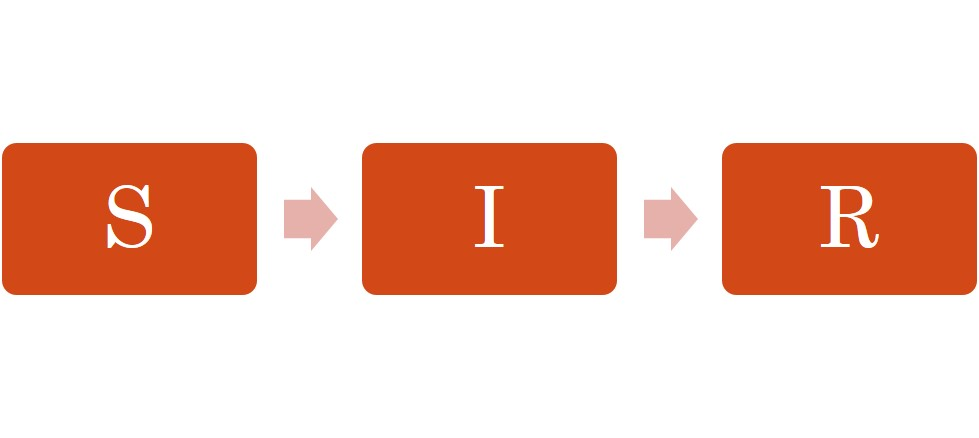
\includegraphics[width= 0.3\textwidth]{./images/SIR-Modell.jpg}\caption{Zustandsmodell des SIR-Modells}
\end{figure}
Das SIR-Modell ist eine mathematische Herangehensweise, bei der der Krankheitsverlauf statisch auf über feste Funktionen errechnet wird. \\
Dazu wird eine geschlossene Gruppe \textbf{N} an Individuen betrachtet. Die Anzahl der Personen in \textbf{N} ist die Gesamtgröße der Bevölkerung. Die Bevölkerung setzt sich aus gesunden, kranken und 'R'-Individuen zusammen, sodass gilt:
\begin{equation}
N = S + I + R
\end{equation}
. Das heißt: Die Bevölkerung wird in drei Zuständen klassifiziert:
\begin{itemize}
\item \textbf{S (Susceptible)} Anfällige Individuen, die innerhalb der Bevölkerung Infiziert werden können.
\item \textbf{I (Infected)} Infizierte Individuen, die Anfällige anstecken  oder in den 'R'-Zustand übergehen können.
\item \textbf{R (Recovered)} Der letzte Zustand ist der \gllqq R \glrqq-Zustand. Ein infiziertes Individuum, was in den \gllqq R\gllqq -Zustand übergeht, bleibt im R-Zustand. Es gibt keinen Übergang aus dem R-Zustand zurück in einen der anderen Zustände. Der R-Zustand kann von daher Individuen beschreiben, die aus Epidemiologischer Sicht keinen Einfluss mehr auf den Rest der Gesellschaft haben. Dies könnten z.B. immunisierte, tote oder isolierte Individuen sein.
\end{itemize}
Zur Visualisierung des Krankheitsverlauf in einer Bevölkerung kann geeigneter Weise ein Koordinatensystem benutzt werden, dass die Anzahl der Individuen in Relation zur Zeit setzt.
Für jede Zustandsgruppe wird ein Graph in das Koordinatensystem gezeichnet, sodass ablesbar wie viele Individuen zu einem Zeitpunkt krank, gesund oder im 'R'-Zustand sind.\\
Die Verteilung der Individuen in die jeweiligen Zustandsklassen ändert sich mit dem Fortschritt der Zeit \textbf{t}, ist die Krankheit nicht ausgestorben, die Infektionsrate oder 'R'-Übergangsrate größer null und nicht alle Individuen im 'R'-Zustand.
Für jeden Zeitschritt wird die Anzahl der Individuen in den Zustandsklassen neu berechnet.\\
Beispielsweise erkranken nach einem Zeitschritt drei neue Individuen und ein Individuum stirbt. Damit nimmt die Gruppe  \textbf{S} um drei Individuen ab, die Gruppe \textbf{I} wächst entsprechend um drei Individuen und gibt gleichzeitig ein Individuum an die Gruppe \textbf{R} ab, sodass sich die Verteilung von beispielsweise S = 5, R = 5 und I = 5 nach einem Zeitschritt zu S = 2, I = 7 und R = 6 ändert.

\subparagraph{Berechnung der Entwicklung mit dem SIR-Modell}
Damit die Verteilung sinnvoll berechnet werden kann, werden Kennzahlen über die Krankheit benötigt, die das Krankheitsprofil widerspiegeln. Dabei wird für das SIR-Modell die Infektionsstärke und die 'R'-Übergangsrate benötigt.
Über die Infektionsstärke $\lambda$ wird die Ansteckung-Kontakt-Rate \textbf{b} ermittelt. Diese ist die Wahrscheinlichkeit mit der ein Individuum, dass mit \textbf{X} Individuen pro Zeitschritt Kontakt hat, erkranken kann.
\begin{equation}
b = ( \lambda * X ) / N
\end{equation}
Dabei ist die Anzahl X der Kontakte pro Zeiteinheit je nach Krankheitsübertragungsweg zu unterscheiden. Bei Krankheiten die über Tröpfcheninfektion übertragen werden, reicht Hände schütteln, die Übergabe von Geld oder sogar das Zusammensein in einem Raum zur Infektion. In diesem Szenario wird oft ein Durchschnittswert von 8 Menschen am Tag genommen.%\cite{}
Bei Krankheiten mit anderen Übertragungswegen z.B. AIDS muss der Austausch von Körperflüssigkeiten zur Infektion stattfinden, d.h. \textbf{X} zeigt den durchschnittlichen Austausch von Körperflüssigkeiten in einem Zeitabschnitt. In diesem Fall ist \textbf{X} im Durchschnitt natürlich deutlich geringer als bei Tröpfcheninfektion.\\
Über die Ansteckungs-Kontakt-Rate kann die Basisreproduktionsrate ermittelt werden. Diese beschreibt die Wahrscheinlichkeit für ein Individuum sich zu infizieren, bei wachsender Anzahl der Menschen im 'R'-Zustand ($\gamma$).
\begin{equation}
R_0 = \frac{ b * N }{ \gamma }
\end{equation}
Hat man die beiden Größen ermittelt, können die Funktionen für die drei Zustände S, I und R über einen Zeitraum ermittelt werden. 
Es gilt:
\begin{equation}
\frac{ \delta S }{ \delta t } = -R_0 * \frac{S * I}{N}
\end{equation}
\begin{equation}
\frac{\delta I }{\delta t} = R_0 * \frac{S * I}{N}
\end{equation}
\begin{equation}
\frac{\delta R }{\delta t} = \gamma * I
\end{equation}

\subparagraph{Warum gerade das SIR-Modell?}
Bei dem Vergleich mit bekannten Modellen aus der Wissenschaft drängt sich zunächst die Frage auf warum im Rahmen des Projektes gerade der Vergleich mit dem SIR-Modell angestellt wird und nicht mit einem anderen Modell zur Darstellung eines Krankheitsverlauf.\\
Wie genau ein mathematisches Modell die Krankheitsausbreitung in einer Gesellschaft beschreibt, hängt sehr davon ab, wie viel Realismus und damit wie viele Annahmen hineingesteckt werden.\\
Da in der Medizin viele Einflüsse zunächst vernachlässigt werden müssen, nicht bekannt sind oder die Krankheit sich mit der Zeit durch mutierende Viren verändert, haben die Modelle sehr selten einen endgültigen Charakter. Darüber hinaus sind Krankheiten in ihrer Entwicklung so unterschiedlich, dass es sehr oft möglich und manchmal nötig ist, die Modelle weiter zu verfeinern und anzupassen, wobei unterschiedliche Krankheiten unterschiedliche Modelle erfordern können. 
\cite{sebM}\\
Mit anderen Worten: Eine Krankheit kann mit all ihren Eigenschaften sehr realitätsnah abgebildet werden, aber möglicherweise bei einer anderen Krankheit schon wieder versagen. Von daher ist nicht das Modell, sondern das zugrunde liegende Szenario entscheidend für die Wahl des Vergleichsmodells. Eine sinnvolle Vorgehensweise ist es daher erst ein Szenario zu erschaffen und dieses dann mit einem geeigneten Modell abzubilden.\\ 
Im Rahmen unserer Projektes wurde sich für die Mittelalterpest entschieden.\\ 
Die Mittelalterpest war im 14. Jahrhundert gleichzusetzen mit einem Todesurteil. Beinahe jedes Individuum erlag nach einiger Zeit seiner Krankheit. Aus diesem Grund passt die Natur des Modells sehr gut zum vorgegebenen Szenario und dem Krankheitsprofil der Pest: Ein gesundes Individuum kann infiziert werden und dann sterben. In diesem Fall bildet der "R"-Zustand, die Anzahl der verstorbenen Individuen ab.\\
Mit einem anderen Szenario wäre es sinnvoll gewesen ein anderes Modell zu betrachten. 
Andere Modelle, die in der mathematischen Biologie angewendet werden sind z.B. das SI-Modell oder SIS-Modell.\\
Das Zustandsmodell im SIS-Modell ist im Gegensatz zum SIR-Modell zyklisch. Es gibt nur zwei Zustände: Anfällig und Infiziert. Anfällige Individuen können infiziert werden und dann wieder genesen. Sind sie genesen können sie wiederum infiziert werden. Damit ist das SIS-Modell vor allem geeignet für bakterielle Erkrankungen wie z.B. Tuberkulose, bei der Individuen wieder genesen, aber keine Immunität entwickeln. \\
\begin{figure}
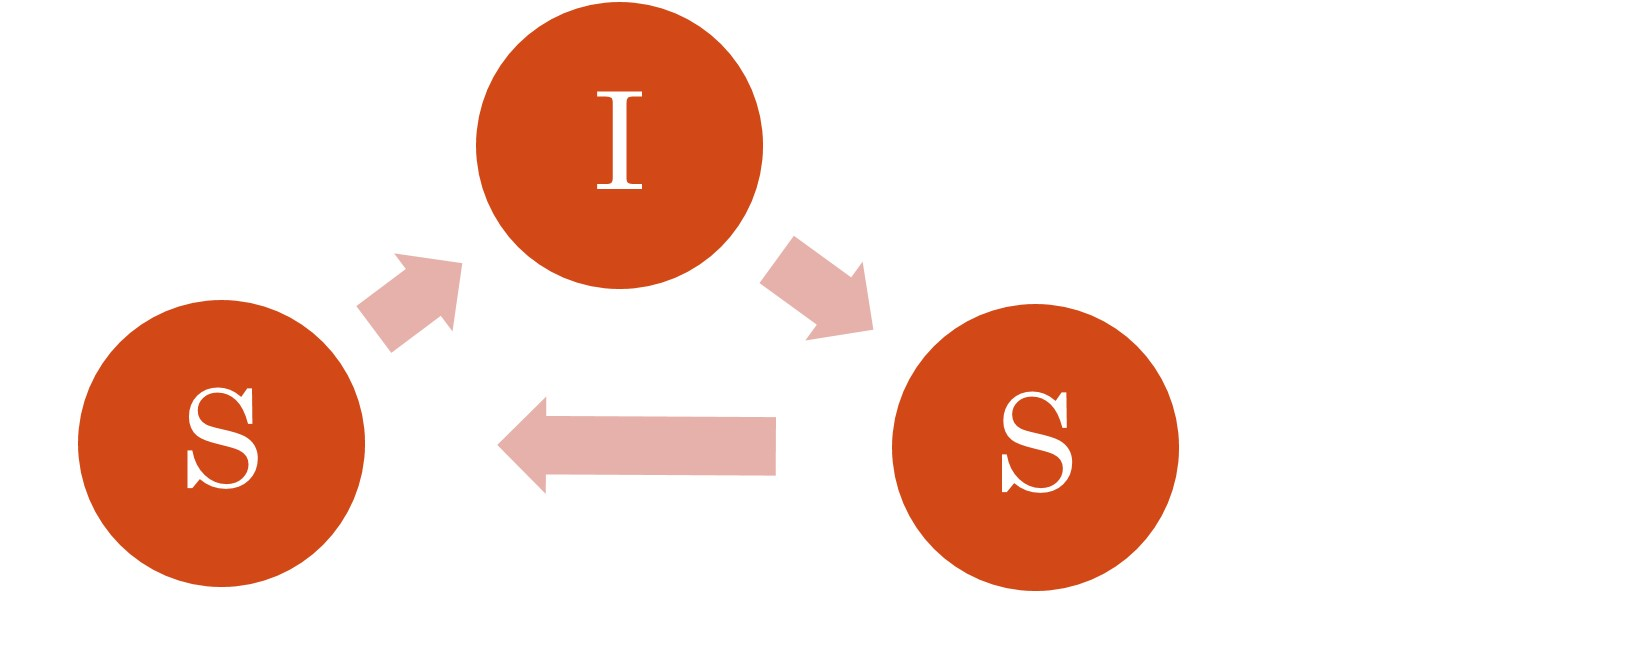
\includegraphics[width= 0.3\textwidth]{./images/SIS-Modell.jpg}\caption{Zuständsmodell des SIS-Modells}
\end{figure}
Das SI-Modell hat ebenfalls die beiden Zustände Anfällig und Infiziert, aber ist nicht zyklisch. Es können lediglich Individuen Infiziert werden. Diese bleiben endgültig im Zustand I.\\ 
Das SI-Modell ist also sinnvoll, wenn Individuen lediglich an einer Krankheit erkranken und nicht wieder genesen, aber auch nicht sterben. Das entsprechende Szenario, wäre beispielsweise ein Zombie-Virus, wie der im Programm implementierte "I am Legend - Virus".\\
Damit wird der erste Vorteil der Herangehensweise im Programm sichtbar: Während bei der mathematischen berechnen für jedes Modell ein anderes Modell gewählt werden muss, um möglichst nah an der Realität zu bleiben, ist das Programm auf mehrere Szenarien mit Heilung, Toten, Resistenten etc. anwendbar.